\section{Sprint 2}

\subsection*{Summary}

\begin{table}[H]
	\centering
	\begin{tabular}{ll}
		\toprule
		\multicolumn{2}{c}{\textbf{Sprint 2}}\\
		\midrule
		\textbf{Periode} & 02.03.2015 12:00 Uhr\textendash 16.03.2015 12:00 Uhr\\
		\textbf{Stunden Soll} & \SI{144}{\hour}\\
		\textbf{Stunden Plan} & \SI{144.3}{\hour} \\
		\textbf{Stunden Ist} & \SI{157.3}{\hour}\\
		\bottomrule
	\end{tabular}
\end{table}

\begin{figure}[H]
	\centering
	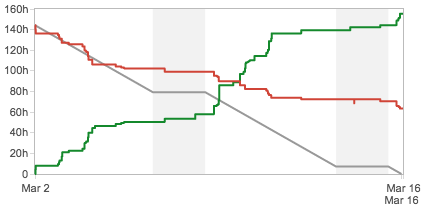
\includegraphics{fig/bd-sprint-2}
	\label{fig:pm:bd-sprint-2}
	\caption*{Burndown Chart Sprint 2}
\end{figure}

\subsection*{Ziele}
Im Hinblick auf die veränderten Umstände der ursprünglichen Aufgabenstellung muss ein Teil der Infrakstruktur neu ausgetzt werden. Zudem stellt sich die Frage nach der groben Architektur des nun selbst zu implementierenden \gls{etl} Prozesses.


\begin{itemize}
	\item Infrakstruktur basierend auf Python aufsetzen
	\item Grobe Architekturüberlegungen für \gls{etl}
	\item Use Cases / User Stories konkretisieren
	\item Erste \gls{hcid} Überlegungen für das Webfrontend
	\item Einarbeitung Django
\end{itemize}

\subsection*{Abgeschlossen}
Folgende High-level (ohne Subtasks) Jira Tasks wurden während Sprint 2 abgeschlossen.

\begin{table}[H]
\centering
\begin{tabular}{ll}
	\toprule
	\textbf{JIRA-Key} & \textbf{Summary}\\
	\midrule
		DAT-14 & Projektmeeting Woche 3\\
		DAT-32 & Sprint 1 Log\\
		DAT-33 & Projektmeeting Woche 4\\
		DAT-34 & Organisation, Planung \& Kommunikation\\
		DAT-36 & Übrige Aufwände Remo Sprint 2\\
		DAT-37 & Übrige Aufwände Christoph\\
		DAT-38 & Übrige Aufwände Fabio\\
		DAT-40 & Epics/User Stories aufnehmen\\
		DAT-41 & Architektur Backend\\
		DAT-43 & HCID\\
		DAT-44 & Django/AngularJS\\
	\bottomrule
\end{tabular}	
\end{table}

\subsection*{Probleme}
Die Einrichtung der Infrastruktur inkl. Continuous Integration und auto-deployment in die Cloud von Heroku hat mehr Zeit beansprucht als ursprünglich geplant.